\documentclass[11pt,a4paper]{article}
\usepackage[utf8]{inputenc}
\usepackage[T1]{fontenc}
\usepackage{amsfonts}
\usepackage[french]{babel}
\frenchbsetup{StandardLists=true} % à inclure si on utilise \usepackage[francais]{babel}
\usepackage{enumitem}
\usepackage{amssymb}
\usepackage{amsmath}
\usepackage[left=2cm,right=2cm,top=2cm,bottom=2cm]{geometry}
\usepackage{multirow}
\usepackage[dvipsnames]{xcolor}

\usepackage[T1]{fontenc}
\usepackage{fouriernc}
\usepackage{graphicx}

\usepackage{setspace}
\singlespacing

\usepackage{pstricks}
\usepackage{xkeyval}
\usepackage{pst-labo}


\usepackage{multicol}
\usepackage{caption}
\usepackage{fancyhdr}
\pagestyle{fancy}
\renewcommand\headrulewidth{1pt}
\fancyhead[L]{Lycée Denis Diderot }
\fancyhead[R]{Classe de 1 Bac Pro }
\setcounter{page}{5}\fancyfoot[C]{page \thepage}
\fancyfoot[R]{Année 2024-2025}
\fancyfoot[L]{Alexis RUIZ}
\usepackage{multirow,tabularx,booktabs}
\usepackage[tikz]{bclogo} 

\newcommand{\cadreblanc}[1]{%
\medskip\framebox[\linewidth][c]{%
\rule{0mm}{#1mm}}\par
\medskip}

\usepackage{awesomebox}
\setlength{\aweboxvskip}{0mm}
\usepackage{pifont}
\usepackage{chemmacros}
\chemsetup{modules=all}
\setlength{\columnseprule}{.25mm}

\renewcommand{\arraystretch}{1.5}
\newcommand*\acocher{\quitvmode{\fboxsep0pt \fboxrule0.8pt \fbox{\vrule height1.8ex depth.1ex width0pt \vrule height0pt depth0pt width1.9ex }}}

\newcolumntype{C}[1]{>{\centering\arraybackslash }b{#1}}

\newcommand{\code}{\awesomebox[black]{2pt}{

\includegraphics[scale=0.15]{images/frame.png}
}{black}}

\newcommand{\moteur}{\awesomebox[black]{2pt}{

\includegraphics[scale=1]{images/moteur.jpg} 
}{black}}

\newcommand{\defconclusion}{\awesomebox[black]{2pt}{\rotatebox{90}{\Large{\textbf{Conclusion}}}}{black}}

\newcommand{\defbox}{\awesomebox[black]{2pt}{
\includegraphics[scale=0.5]{images/appel exam.png}}{black}}

  \newenvironment{itemize*}%  % listes compactes
    {\begin{itemize}%
      \setlength{\itemsep}{0pt}%
      \setlength{\parskip}{0pt}}%
    {\end{itemize}}

\frenchbsetup{StandardLists=true}



\begin{document}

\flushleft \textbf{NOM : \hfill Classe : \hspace{3cm} ~~\\[2mm]
Prénom:\\[0,4cm]
}
\hrule\
\\[0,2cm]

\begin{center}
 \LARGE{TP1  - Comment calculer la puissance électrique consommée par une lampe de voiture ?  }
\end{center}

\vspace{3 mm}

\normalsize

\hrule\
\\[0,2cm]
   \begin{center}
   \textbf{Le soin et la rédaction interviendront dans la notation.}
   \end{center} 

\noindent%
\begin{minipage}{.5\textwidth}%

    
 \begin{bclogo}[couleur=blue!30 ,  arrondi =0.1 , logo = \bcinfo, epBarre =2]{ Matériel }

\begin{itemize*}
    \item 1 lampe 
    \item 1 voltmètre
    \item 1 ampéremètre
    \item 1 générateur 12V CC
    \item 5 fils de connexion
\end{itemize*}
\end{bclogo}

\end{minipage}%
\hfill
\begin{minipage}{.30\textwidth}%
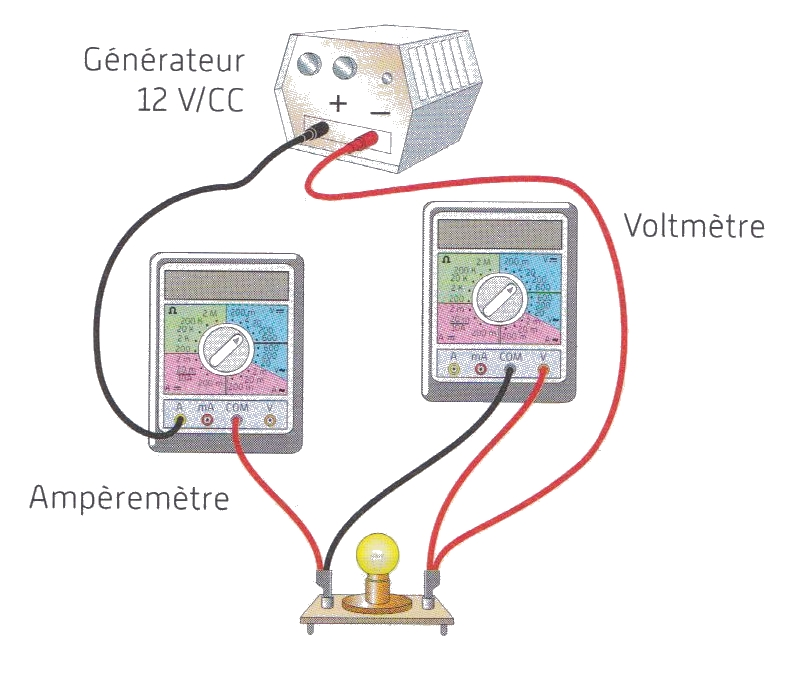
\includegraphics[width=\textwidth]{images/TP2 - Montage.png}
\end{minipage}%



\fcolorbox{black}{blue!30}{\textbf{Protocole}}
\begin{itemize*}
    \item Relevez sur la lampe puis écrire dans le tableau ci-dessous, sa tension nominale $U_N$ en volts et sa puissance nominale \textbf{$P_N$} , en W, données par le fabricant.
    \item Réaliser le montage électriques ci-dessus.

\defbox{\fbox{
\begin{minipage}{8cm}{

Appeler M Ruiz pour qu'il vérifie le montage.}

\end{minipage}
}}


    \item Allumez la lampe.
    \item Relevez puis écrire dans le tableau ci-dessous les valeurs $U (en V)$ , $I (en A)$
    \item Finissez de complétez le tableau suivant 
\end{itemize*}



\fcolorbox{black}{blue!30}{\textbf{Mesures}}\\
\ding{202} Complétez le tableau suivant : 

\begin{center}
    

    \begin{tabular}{|C{2cm}|C{2cm}||C{2cm}|C{2cm}||C{2cm}|}
         \hline
         Tension & Puissance &  Tension mesurée & Intensité mesurée & Produit\\
         
         $U_N (V)$ & $P_N (W)$ & $U (V)$  & $I (A)$ & $U \times I$ \\
         \hline
           &  &  &  & \\
         \hline
 
    \end{tabular}
\end{center}




\fcolorbox{black}{blue!30}{\textbf{Interprétation }} \\[5mm]
\ding{202} Comparez le produit $U \times I$ à la puissance nominale $P_N$ de la lampe\\
\vspace{3mm}
\dotfill 





\fcolorbox{black}{blue!30}{\textbf{Validation}}\\[5mm]
\begin{multicols}{2}

\ding{207}  Calculez l'erreur relative en utilisant la formule : 
\begin{multicols}{2} 
\begin{center}
    
$e_a= \dfrac{P_N - U \times I}{P_N}$ \end{center}
   \cadreblanc{10}
\end{multicols}
\ding{208} Conclure en écrivant la relation liant $P$, $U$ et $I$. 
\vfill 
   \cadreblanc{10}

\end{multicols}





\end{document}